% Данный файл распространяетсяя под лицензией CC BY 4.0. Текст лицензии размещён на https://creativecommons.org/licenses/by/4.0/
% (c) Кафедра системного программирования, 2025

\documentclass[a4paper]{article}

\usepackage[a4paper, top=8mm, bottom=8mm, left=8mm, right=8mm]{geometry}

\usepackage{polyglossia}
\setdefaultlanguage[babelshorthands=true]{russian}
\setotherlanguage{english}

\usepackage{fontspec}
\setmainfont{FreeSerif}
\newfontfamily{\russianfonttt}[Scale=0.7]{DejaVuSansMono}

\usepackage[tiny, compact]{titlesec}

\usepackage{titling}
\setlength{\droptitle}{-1cm}
\pretitle{\begin{center}\begin{bfseries}\Large}
\posttitle{\par\end{bfseries}\end{center}}
\preauthor{\begin{center}\normalsize}
\postauthor{\par\end{center}\vspace{-1.8cm}}

\usepackage{hyperref}
\usepackage{bookmark}
\usepackage{csquotes}
\usepackage{graphicx}
\usepackage[table]{xcolor}
\usepackage{url}
\usepackage{float}

\title{Vortex: освоение FPGA-стека}

\author{Правкин Даниил Денисович}

\date{}

\begin{document}

\maketitle

\begin{flushright}
    Группа: \enquote{25.Б73-мм}

    Кафедра: системного программирования


    Научный руководитель: Григорьев Семён Вячеславович

    
    Номер семестра практики: 2
\end{flushright} 


\section{Введение}

Графический процессор (GPU)~--- вычислительный блок, созданный для ускорения параллельных операций при 3D-рендеринге в реальном времени. Большинство его транзисторов используется для обработки данных, в то время как в центральном процессоре (CPU) значительная часть задействована для кэширования и управления потоками. За счёт этого GPU обеспечивает более высокую скорость обработки команд и пропускную способность памяти, чем CPU, при аналогичных цене и мощности~\footnote{Информация взята из CUDA Pragramming Guide, URL: \url{https://docs.nvidia.com/cuda/archive/13.1.0/cuda-programming-guide/01-introduction/introduction.html} (дата обращения: 13.06.2026).}.

Vortex~--- это проект с открытым исходным кодом, предназначенный для поддержки вычислений на графических процессорах (GPGPU). Он реализован на основе расширений системы команд RISC-V ISA и предусматривает возможность аппаратной конфигурации. Vortex использует модель исполнения SIMT (Single Instruction Multiple Threads)~\footnote{Документация Vortex о микроархитектуре, URL: \url{https://github.com/vortexgpgpu/vortex/blob/master/docs/microarchitecture.md} (дата обращения: 27.04.2026).}, в рамках которой одна и та же инструкция выполняется над разными данными. Это достигается при помощи потоков (threads)~--- наименьших единиц вычисления, выполняемых параллельно,~--- и варпов (warps), которые представляют собой набор потоков, исполняющих одну и ту же инструкцию. За счёт этого достигается распараллеливание выполнения задачи. Одной из задач, выполняемой при помощи такой модели исполнения, является умножение матриц (например, в графических процессорах от компании NVIDIA)~\footnote{В архитектуре CUDA, использующей SIMT, также есть функция умножения матриц, URL: \url{https://docs.nvidia.com/cutlass/latest/media/docs/cpp/efficient_gemm.html} (дата обращения: 29.05.2026).}.

Результаты работы необходимы для дальнейшей работы с Vortex: сборка Vortex, оценка потребления ресурсов конфигурации, сравнение различных конфигураций.

\section{Постановка задачи}

Целью данной работы является получение навыков работы с FPGA-стеком.

Для достижения цели требуется решить следующие задачи:
\begin{enumerate}
    \item выполнить обзор способов симуляции Vortex;
    \item провести эксперименты с функцией умножения матриц при различных конфигурациях Vortex.
\end{enumerate}

\section{Обзор}

Перед проведением экспериментов необходимо было выбрать способ симуляции Vortex: RTL-симуляцию или Cycle-Approximate-симуляцию.

Первый вариант осуществляется при помощи Verilator~--- симулятора, преобразующего код на Verilog HDL в однопоточный или многопоточный код на C++/SystemC. В таком подходе моделируется каждый отдельный сигнал, триггер и логический элемент. Вследствие чего данный метод довольно точен, но при этом затрачивает много времени.

Второй вариант осуществляется при помощи SimX~--- симулятора Vortex, написанного на C++. Он является потактовым, то есть воспроизводит поведение микроархитектуры с точностью до такта (содержимое кэша, состояние счётчиков, загрузка конвейера). Поэтому данный метод чуть менее точен, но более быстр по сравнению с RTL-симуляцией.

Поскольку эксперимент предполагает многократный запуск тестов и анализ общего поведения функции, а не получение абсолютно точного значения затраченных тактов, для сокращения временных затрат было принято решение использовать в экспериментах симулятор SimX.

\section{Описание предлагаемого решения}

С целью получения навыков работы с Vortex был проведён эксперимент по измерению масштабируемости функции умножения матриц. Реализация решения осуществлялась в среде Docker-контейнера с применением симулятора SimX.

\section{Эксперименты}

\subsection{Цель}
Проанализировать масштабируемость функции умножения матриц при увеличении количества ядер и фиксированном объёме входных данных.

\subsection{Условия эксперимента}
\samepage{
    Во время эксперимента использовались:
    \begin{itemize}
        \item Vortex 2.2
        \item Docker Engine 29.5.2
    \end{itemize}
}

Для экспериментов была выбрана матрица размера $512\times512$ с целью получения более реалистичной производительности. Для алгоритма требуется память для двух перемножаемых матриц и одной итоговой, при этом каждый элемент матрицы имеет тип float~\footnote{Информация из реализации функции sgemm в Vortex, URL: \url{https://github.com/vortexgpgpu/vortex/blob/master/tests/regression/sgemm/common.h} (дата обращения: 12.06.2026).}, следовательно, объём трёх матриц данного размера~--- 3~МиБ, что превышает объём общей памяти (Local Memory) (128 КиБ), L1-кэша (16~КиБ), L2-кэша (1~МиБ) и L3-кэша (2~МиБ)~\footnote{Объёмы общей памяти и l1/l2/l3-кэшей взяты из документации Vortex (объём общей памяти: URL: \url{https://github.com/vortexgpgpu/vortex/blob/master/hw/rtl/mem/VX_local_mem.sv}, оъёмы кэшей: URL: \url{https://github.com/vortexgpgpu/vortex/blob/master/docs/simulation.md}) (дата обращения: 26.04.2026).}; следовательно, программа будет больше взаимодействовать с основной памятью.

\samepage{
    Порядок выполнения экспериментов:
    \begin{enumerate}
        \item отключение графической оболочки, для повышения скорости симуляции;
        \item запуск Docker-контейнера;
        \item запуск тестов и запись результатов.
    \end{enumerate}
}

Сперва надо было подобрать оптимальную конфигурацию для более реалистичной производительности. Подбор производился при cores=8, потому что большее количество ядер порождает большую нагрузку на память, то есть более реалистичную производительность.

Далее запускались тесты с оптимальной конфигурацией, но изменяемым количеством ядер. Значения количества ядер кратны степеням двойки, чтобы обеспечить более равномерное распределение нагрузки между ядрами, так как размер матрицы тоже кратен степени двойки.

\subsection{Результаты}

В результате поиска аппаратной конфигурации (табл.~\ref{tab:optimal_for_8}) наиболее оптимальной при восьми ядрах оказалась следующая: clusters=1, warps=8, threads=64, l2cache, l3cache.

По результатам эксперимента по измерению масштабируемости (рис.~\ref{figure:sgemm_graph}), при увеличении числа ядер от 1 до 16 количество тактов уменьшается, а при cores=16 достигает наименьшего значения. В диапазоне от 17 до 31 в ходе экспериментов возникали ошибки, свидетельствовавшие о неудачной попытке разделить задачу между всеми вычислительными блоками. Например, при запуске конфигурации с 18~ядрами в итоговой статистике для двух из них были выведены отрицательные значения количества выполненных инструкций и затраченных тактов. При дальнейшем увеличении числа ядер (начиная с 32) наблюдался рост количества тактов. Это свидетельствует о накладных расходах, затрачиваемых на корректную работу вычислительных блоков, в том числе для обеспечения параллельного выполнения, вследствие чего суммарное количество превышает значение, полученное при 16~ядрах. Таким образом, для умножения матриц $512\times512$ при фиксированных параметрах (clusters=1, warps=8, threads=64, l2cache, l3cache) наименьшее количество тактов достигается при использовании 16~ядер.

\begin{table}[h]
    \centering
    \caption{\label{tab:optimal_for_8} Число тактов, затраченных на выполнение алгоритма умножения матриц размера $512\times512$ при фиксированных параметрах (cores=8, clusters=1, l2cache, l3cache) и различных значениях числа потоков и групп потоков. Выделенная строка~--- конфигурация, при которой затрачено наименьшее число тактов.}
    \begin{tabular}{r r r}
        \hline
        \multicolumn{1}{c}{Кол-во групп потоков} & \multicolumn{1}{c}{Кол-во потоков} & \multicolumn{1}{c}{Кол-во тактов (млн.)} \\ \hline
        2 & 16 & 43,0 \\ \hline
        2 & 32 & 22,8 \\ \hline
        2 & 64 & 13,8 \\ \hline

        4 & 16 & 30,3 \\ \hline
        4 & 32 & 16,4 \\ \hline
        4 & 64 & 13,7 \\ \hline

        8 & 16 & 30,6 \\ \hline
        8 & 32 & 18,8 \\ \hline
        \rowcolor{lightgray}
        8 & 64 & 13,6 \\ \hline

        16 & 16 & 33,4 \\ \hline
        16 & 32 & 18,8 \\ \hline
        16 & 64 & 14,2 \\ \hline
    \end{tabular}
\end{table}

\begin{figure}
    \centering
    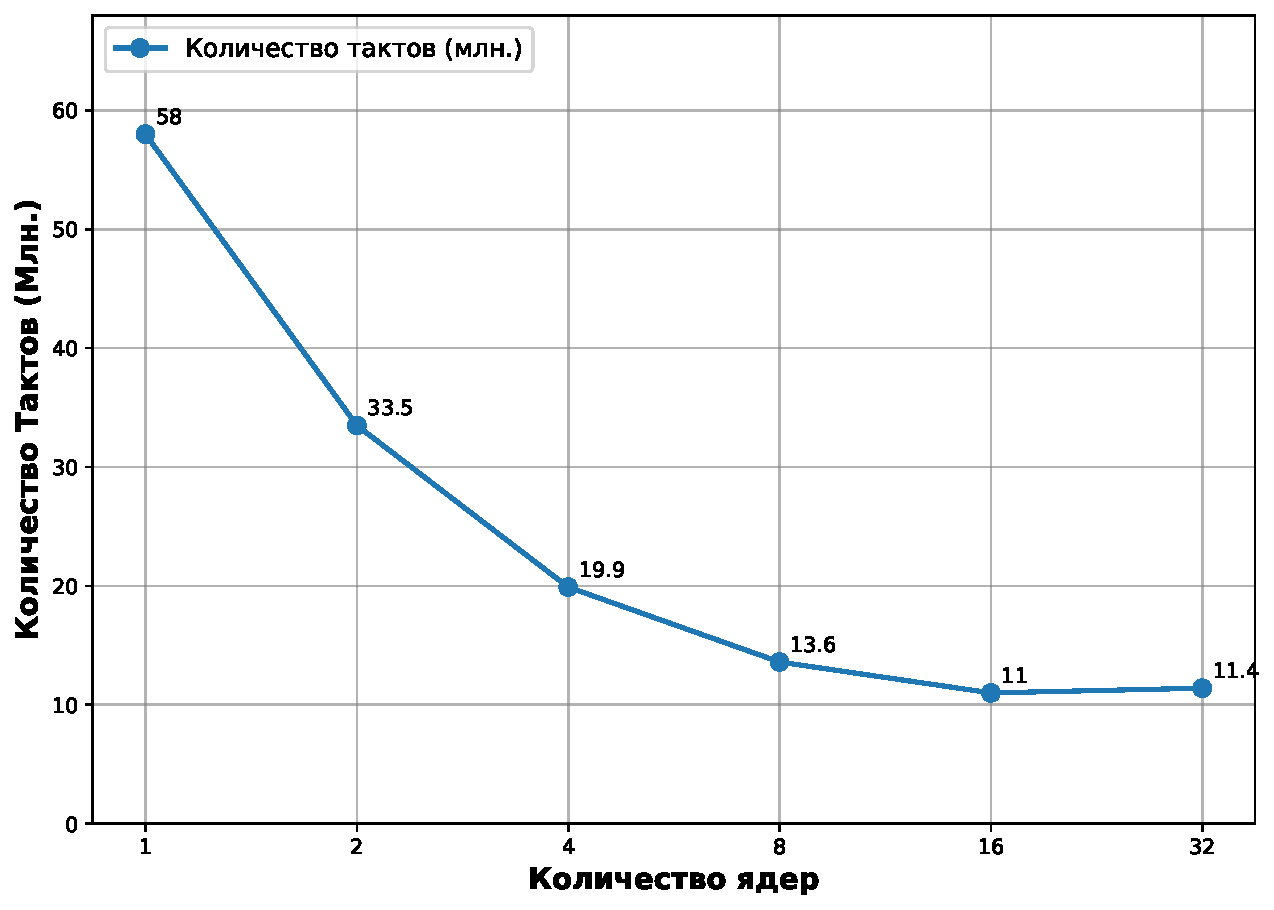
\includegraphics[width=0.8\linewidth]{sgemm_graph.pdf}
    \caption{\label{figure:sgemm_graph} Изменение числа тактов, затраченных на выполнение алгоритма умножения матриц при фиксированных параметрах (clusters=1, warps=8, threads=64, l2cache, l3cache) и различных значениях количества ядер.}
\end{figure}


\section{Заключение}

В ходе выполнения работы получены следующие результаты:

\begin{itemize}
    \item произведено сравнение количества тактов, затрачиваемых различными конфигурациями Vortex при выполнении функции умножения матриц;
    \item проанализирована масштабируемость функции умножения матриц.
\end{itemize}

Техническая документация: \url{https://github.com/Prosto-Dan/vortex_practice_1_year/blob/main/docs/analyze.md}.

\end{document}
